% Number 90
% CAPM GMM
% v graphs - conceptual q
% MIT Physics for Teachers LON-CAPA

% Watermark
\AddToShipoutPicture*{\BackgroundPic}

\addtocounter {ProbNum} {1}

\begin{floatingfigure}[r]{.3\textwidth}
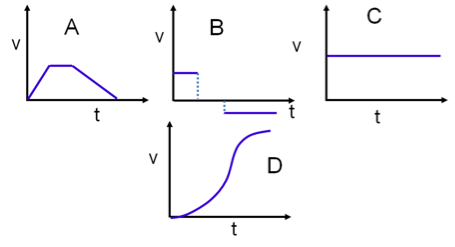
\includegraphics[scale=.4]{/Users/jgates/desktop/latex/pics/vgraph1.png}
\end{floatingfigure}
 
{\bf \Large{\arabic{ProbNum}}} A car starting from rest speeds up to ${30~\frac{m}{s}}$ with constant acceleration in 10 seconds. Then, it travels at ${30~\frac{m}{s}}$ for 10 seconds. Finally, it brakes to a stop in 20 seconds with constant acceleration. 
\bigskip

\indent Which of the following graphs represents the speed of the car versus time?  
 

\vfill

\newpage
